\section{Command in terminal}

\textbf{See the command usage and information}
\begin{lstlisting}[style=bashStyle]
    $ man {command}
\end{lstlisting}
\text{Example:}
\begin{lstlisting}[style=bashStyle]
    $ man insmod
\end{lstlisting}
\text{Result}
\begin{center}
    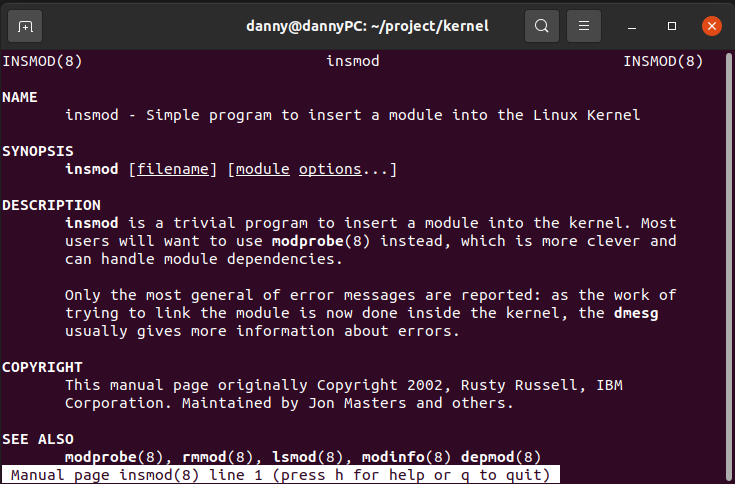
\includegraphics[width=\linewidth]{images/man_insmod.png}
\end{center}

\textbf{Insert a kernal module}
\begin{lstlisting}[style=bashStyle]
    $ sudo insmod {module name (*.ko)}
\end{lstlisting}

\textbf{Show a kernal module info}
\begin{lstlisting}[style=bashStyle]
    $ sudo modinfo {module name (*.ko)}
\end{lstlisting}

\textbf{Print or control the kernel ring buffer}
\begin{lstlisting}[style=bashStyle]
    $ sudo dmesg
\end{lstlisting}

\textbf{Simple program to remove a module from the Linux Kernel}
\begin{lstlisting}[style=bashStyle]
    $ sudo rmmod {module name}
\end{lstlisting}


\textbf{Add and remove modules from the Linux Kernel}

Loads the module only in /lib/modules/`uname -r`
modprobe depends on depmod tool to calculate dependancies
\begin{lstlisting}[style=bashStyle]
    $ sudo modprobe {module name}
    $ echo the dependancies
    $ vi /lib/module/`uname -r`/modules.dep
\end{lstlisting}









